
\documentclass{beamer}
\usepackage{natbib}

\title{Measuring Income Tax Evasion Using Bank Credit: Evidence from Greece Get access Arrow by \citet{artavanis2016measuring}}
\author{}
\date{\today}
\begin{document}

\frame{\titlepage}

\begin{frame}
\frametitle{Some Odd Patterns in Bank Loans}
\begin{figure}
    \centering
    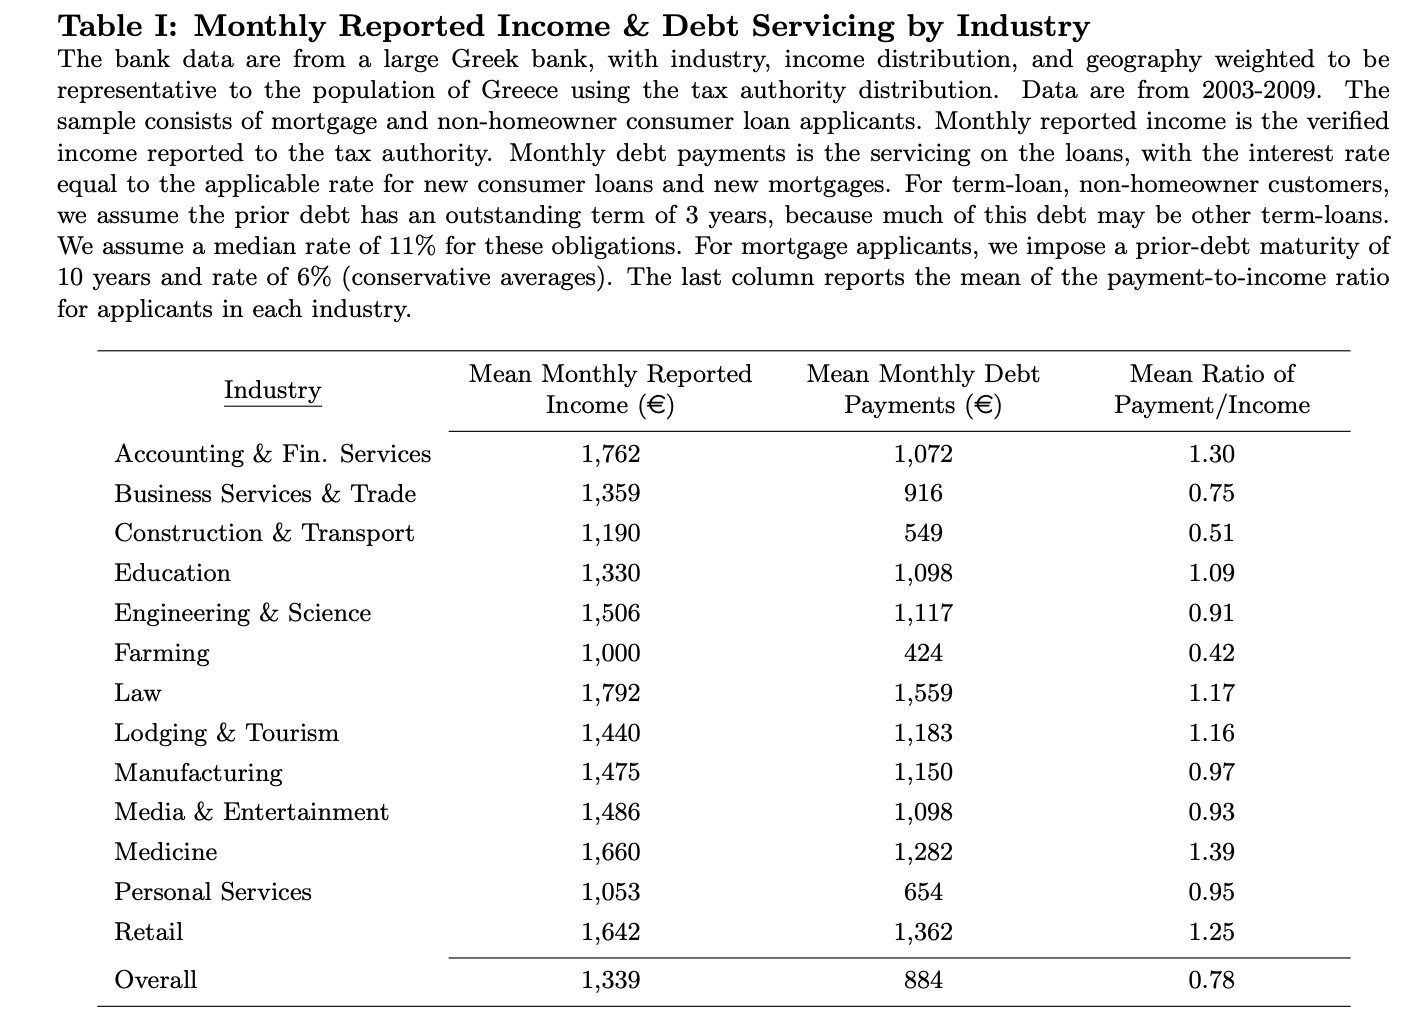
\includegraphics[width=\textwidth]{Paper Presentations/Table1.png}
\end{figure}
\end{frame}


\begin{frame}
\frametitle{Stylized Facts }
\begin{itemize}
    \item Effective global capital income taxes have increased since 1995 due to hyper-globalization. 
    \item By increasing the concentration
of economic activity in formal corporate structures relative to smaller informal businesses, trade liberalization facilitates the imposition of taxes, particularly of corporate taxes.
\item Trade liberalization can explain 18-41\% of the
rise in effective capital tax rates in developing countries.
\end{itemize}
\end{frame}

\begin{frame}{Methods}
\begin{itemize}
\item Effective tax rate of any factor is total taxes collected on that factor divided by the income of that factor. 
\item The challenge is how to measure labor income, capital income and taxes paid. One needs to allocate both income and taxes paid to these two factors. 
\item You will have to assign a portion of each type of tax revenue to one of two factors. 
\begin{enumerate}
    \item Corporate income, wealth, and property taxes are allocated to capital. 
    \item Payroll and social taxes are allocated to labor. 
    \item Personal Income taxes are allocated to both in country-time specific manner.
\end{enumerate}
\item Net GDP is decomposed into labor and capital income, where 
\[Y_L = CE+ \phi.OS_{PUE} \]
\[Y_K = (1-\phi) . OS_{PUE}+OS_{CORP}+ OS_{HH}\]

\end{itemize}
\end{frame}

\begin{frame}{Trade offs}
\begin{itemize}
    \item SS can be implemented under weaker assumptions. 
    \item What it actually identifies is credible and transparent. 
    \item We can always use SS even when we are not exactly sure about the model that generates this behaviour. 
    \item But you always need a formula for every economic question. It does not capture every aspect of the model. 
    \item This also cannot help with out of sample predictions in comparison to structural models.
\end{itemize}    
\end{frame}

\begin{frame}
\frametitle{Methodology}
\begin{itemize}
    \item Framework of the sufficient-statistic approach.
    \item Key formulas and models.
\end{itemize}
\end{frame}

\begin{frame}
\frametitle{Applications}
\begin{itemize}
    \item Application in income taxation.
    \item Application in social insurance.
\end{itemize}
\end{frame}

\begin{frame}
\frametitle{Behavioral Models}
\begin{itemize}
    \item Application to behavioral economics.
\end{itemize}
\end{frame}

\begin{frame}
\frametitle{Broader Implications}
\begin{itemize}
    \item Potential applications in various economic fields.
\end{itemize}
\end{frame}

\begin{frame}
\frametitle{Conclusion}
\begin{itemize}
    \item Main findings and contributions.
    \item Importance in policy analysis.
\end{itemize}
\end{frame}

\begin{frame}{Bibliography}
\bibliographystyle{plainnat}
\bibliography{Paper Presentations/bib}
\end{frame}

\end{document}
